\documentclass[conference, onecolumn]{IEEEtran}
% Include all packages from file.
% Report template for Mälardalen University
% Original template can be found: 
% https://www.overleaf.com/latex/templates/ieee-bare-demo-template-for-conferences/ypypvwjmvtdf
% Template file structure organised by: Emil Persson
% The following packages should follow the IEEE conference guidelines.

% Swedish language package 
\usepackage[utf8]{inputenc}
\usepackage[T1]{fontenc}
\usepackage[swedish,english]{babel}

% Graphics
\usepackage{graphicx, float, subfigure, blindtext}

\newcommand\IEEEhyperrefsetup{
bookmarks=true,bookmarksnumbered=true,%
colorlinks=true,linkcolor={black},citecolor={black},urlcolor={black}%
}

% Preferred hyperref setup, Michael Shell
\usepackage[\IEEEhyperrefsetup, pdftex]{hyperref}

% Maths
\usepackage{mathtools}

% These packages must be at the end
\usepackage[nolist,nohyperlinks]{acronym}
\usepackage{cleveref}
\graphicspath{{images/}}

% Remove section first paragraph indent
\usepackage{titlesec}
\titlespacing*{\section}{0pt}{*1}{*1}
\titlespacing*{\subsection}{0pt}{*1}{*1}
\renewcommand{\thesubsubsection}{\arabic{subsubsection}}
\titleformat{\subsubsection}[runin]{\itshape}{\thesubsubsection)}{1em}{}[:]
\titlespacing*{\subsubsection}{\parindent}{0pt}{*1}

% Include authors 
\author{\IEEEauthorblockN{ %
Ashley Björs\IEEEauthorrefmark{1}
}
\IEEEauthorblockA{
School of Innovation, Design and, Engineering\\
Mälardalens University, Västerås, Sweden, 2024-10-04\\
Email:
\IEEEauthorrefmark{1}abs21004@student.mdu.se,
}}

% ACRONYMS: \acrodef{acronym}[short name]{full name}
\acrodef{svm}[SVM]{Support Vector Machine}

% The report title.
\title{ELA212 Instuderings frågor}
% Document begins here
\begin{document}
% Create the title.
\maketitle
% Example sections, name them
% according to specific needs.
\section{Threshold and color space}
\subsection{How did you create the filter? Did you get a good result, i.e. like the middle image of Figure 1? Why/why not? (Possibly there is a lot of white pixels – do not worry).}
By changing any value in the green colour channel which fell below 0.5 to 0 and everything else to 1 a basic highpass filter was made. The quality of said filter was less than ideal due it not being able to differentiate between green and any colour which has sufficiently high green components e.g. white.

%By hemming in the colour space of the Red, Green \& Blue bands as little of the desired values were removed. It is not ideal and parts of the scene has parts which contain the RGB spans even if it does not look "green"
\subsection{Suggest how to improve the result.}
By switching from RGB to HSV we could pick out a pure colours instead of any colour with sufficient high concentration of a basic colour.
\subsection{How do you create the green filter in this color space? Which parameter was the most important?}
Due to there being few items in the scene with similar hues and the bag being fairly uniformly coloured it can easily be cut out in the HSV view. The Hue was deemed to be most significant when filtering for the green bag while saturation and value was less impactful.
\subsection{How does your filtered image compare to the previous RGB-based result?}
Massivly improved and most white specks are removed leaving only the bag.
\subsection{How did you do this?}
We spun the RGB values clockwise within the mask which contained the bag. Turning Red to Green, Green to Blue and Blue to Red. This could have been done in the HSV but the image was already in RGB.
\subsection{Show the resulting image}
See figure 1
\begin{figure}[h]
    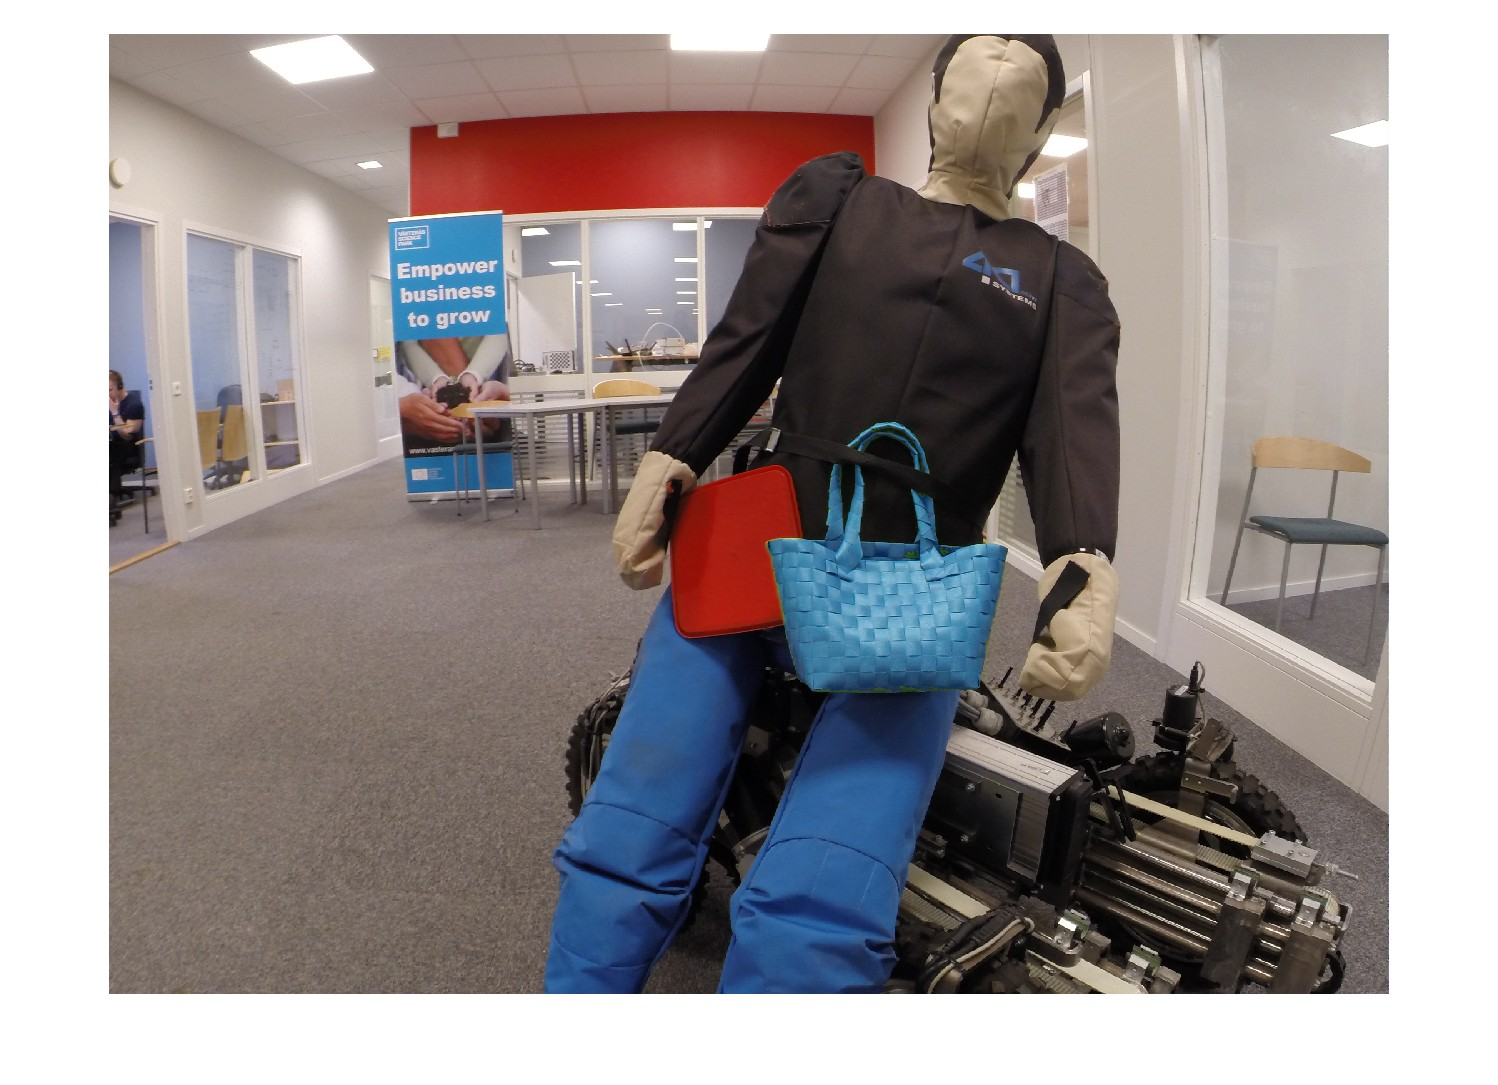
\includegraphics[width=\textwidth]{./bluebag.jpg}
    \caption{A picture of bob with a colour swapped bag}
\end{figure}
\section{Spatial operator and convolution}
\subsection{Compare A=(I*s)*g and B=I*(s*g). Do they produce the same result?}
Yes the images are indestinguisable due to the order the convolutions are done in is irrelevant for the resulting image.
See figure 2
\begin{figure}[h]
    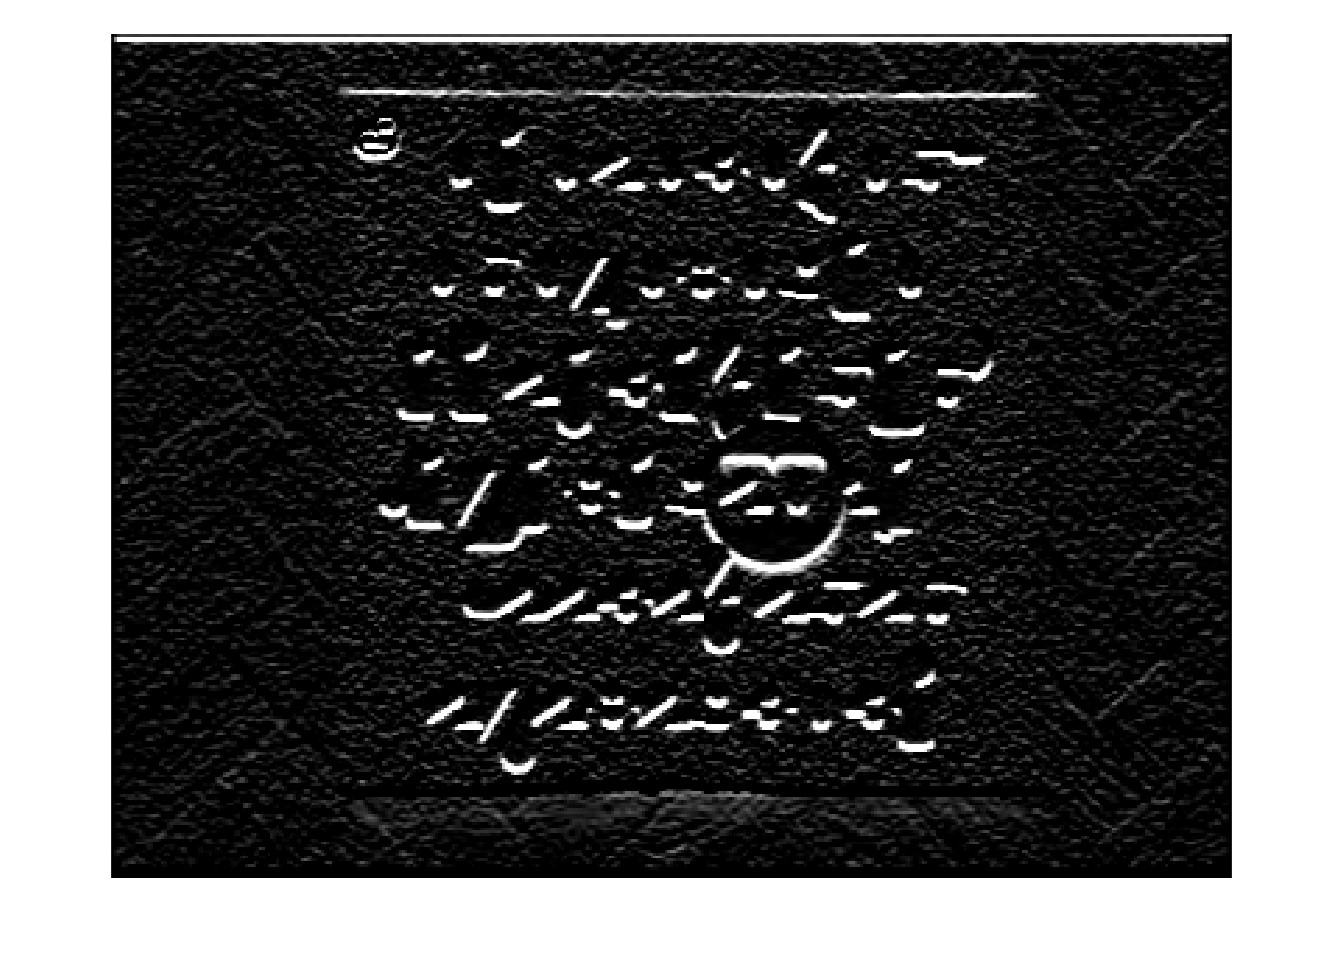
\includegraphics[width=0.5\textwidth]{./Conv((Cs)g).jpg}
    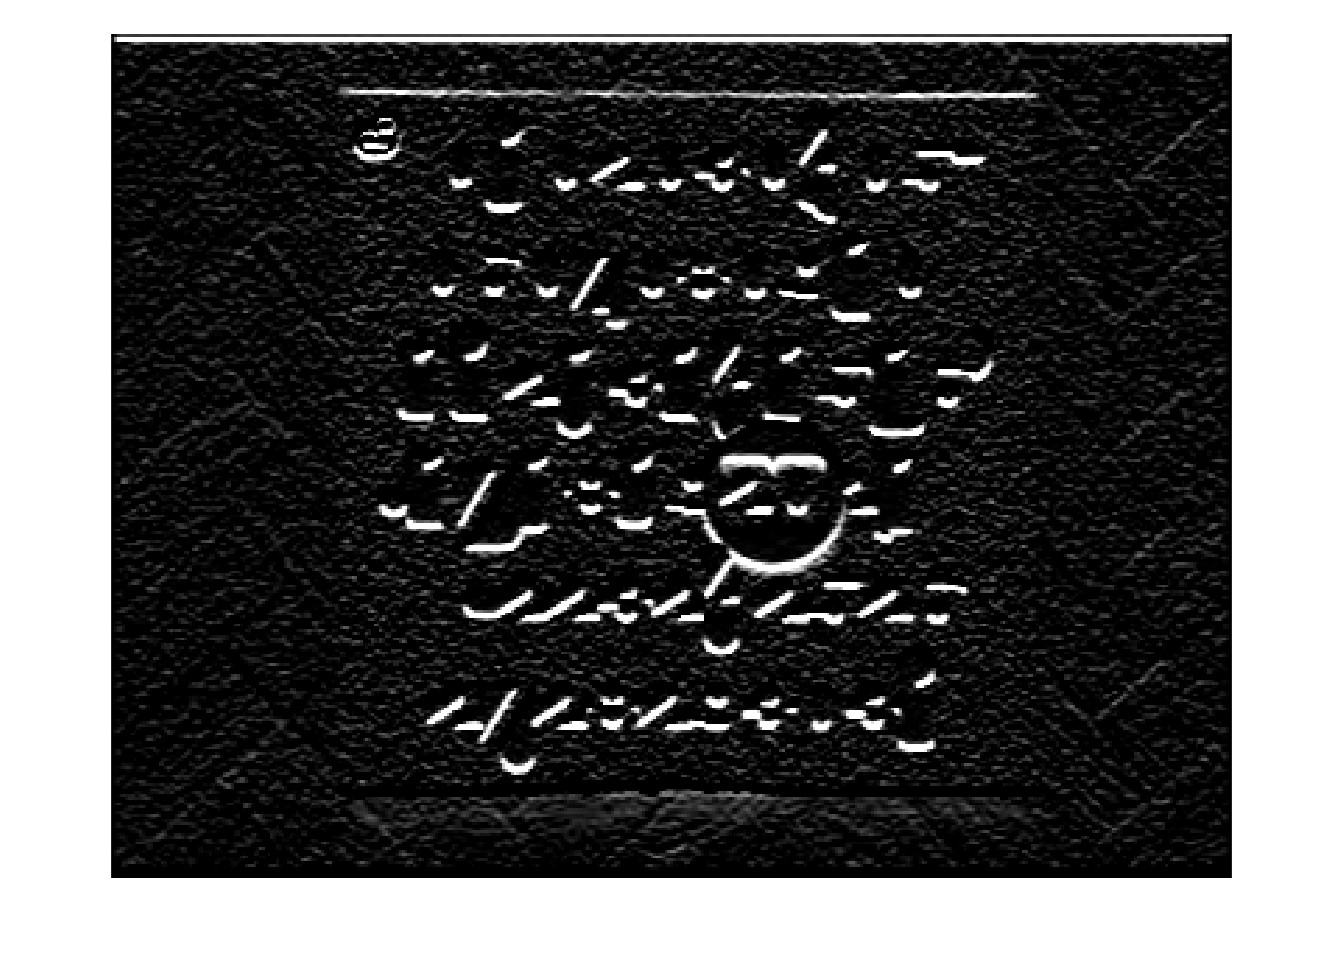
\includegraphics[width=0.5\textwidth]{./Conv(C(sg)).jpg}
    \caption{The image A is on the left and image B is on the right}
\end{figure}


\subsection{Which one is quicker and why? Use tic, toc. Note: As the image is small loop the operation to get a better time estimation}
image A took 0.556078s for 1000 iterations

image B took 0.190311s for 1000 iterations

B is faster due it only having to do convolutions including the larger matrix once per iteration.
\section{Calibration and measurement}
\subsection{What was the result of your 4 depth estimations? What do you conclude from these with respect to measurement and distortion?}
Disrtorted Pen1 distance was estimated to be 387mm away

Disrtorted Pen2 distance was estimated to be 427mm away

Undisrtorted Pen1 distance was estimated to be 385mm away

Undisrtorted Pen2 distance was estimated to be 378mm away

Human error of picking the pixels are a way larger factor than the undistortion function corrects. The two undistorted distances are closer to eachother and can be assumed to be more accurate. Visually the undistorted images look subjectivly better around the center of the image.

% \input{sections/abstract}
% \input{sections/keywords}
% \input{sections/introduction}
% \input{sections/method}
% \input{sections/results}
% \input{sections/discussion}
% \input{sections/conclusion}
% \input{sections/acknowledgement}
% Select the IEEEtran style
\bibliographystyle{IEEEtran}
% Include bibliography file
\bibliography{IEEEabrv,refs}
\end{document}